\chapter{Arkitektur}\label{ch:Arkitektur}

Designet af arkitekturen har en indflydelse på forståelsen af systemet er organiseret, samt softwarens struktur. Specielt når det gælder den agile tilgang, er software design noget der bliver fokuseret på i starten af processen, da inkrementel udvikling af arkitektur vil ofte give vanskeligheder. Det samme gælder andet som refactoring og arkitektur. Dette vil ende ud i forsinkelse af systemet, netop fordi systemet skal modificeres relativt meget for at tilpasse dig forandringerne. Derfor er arkitekturen en proces, som gerne skal fasslåes i starten af et software projekt. \cite{Sommerville}

Til dette, har gruppen forudbestemt, inden implementering af systemet, hvordan arkitekturen skal se ud. Her har der været fokus på udelukkende en domæne-model og en relations model, da disse 2 vil give det bedste udtryk af, hvordan software er designet. Hertil en model for hvordan system arkitekturen er opast. 

\begin{figure}
    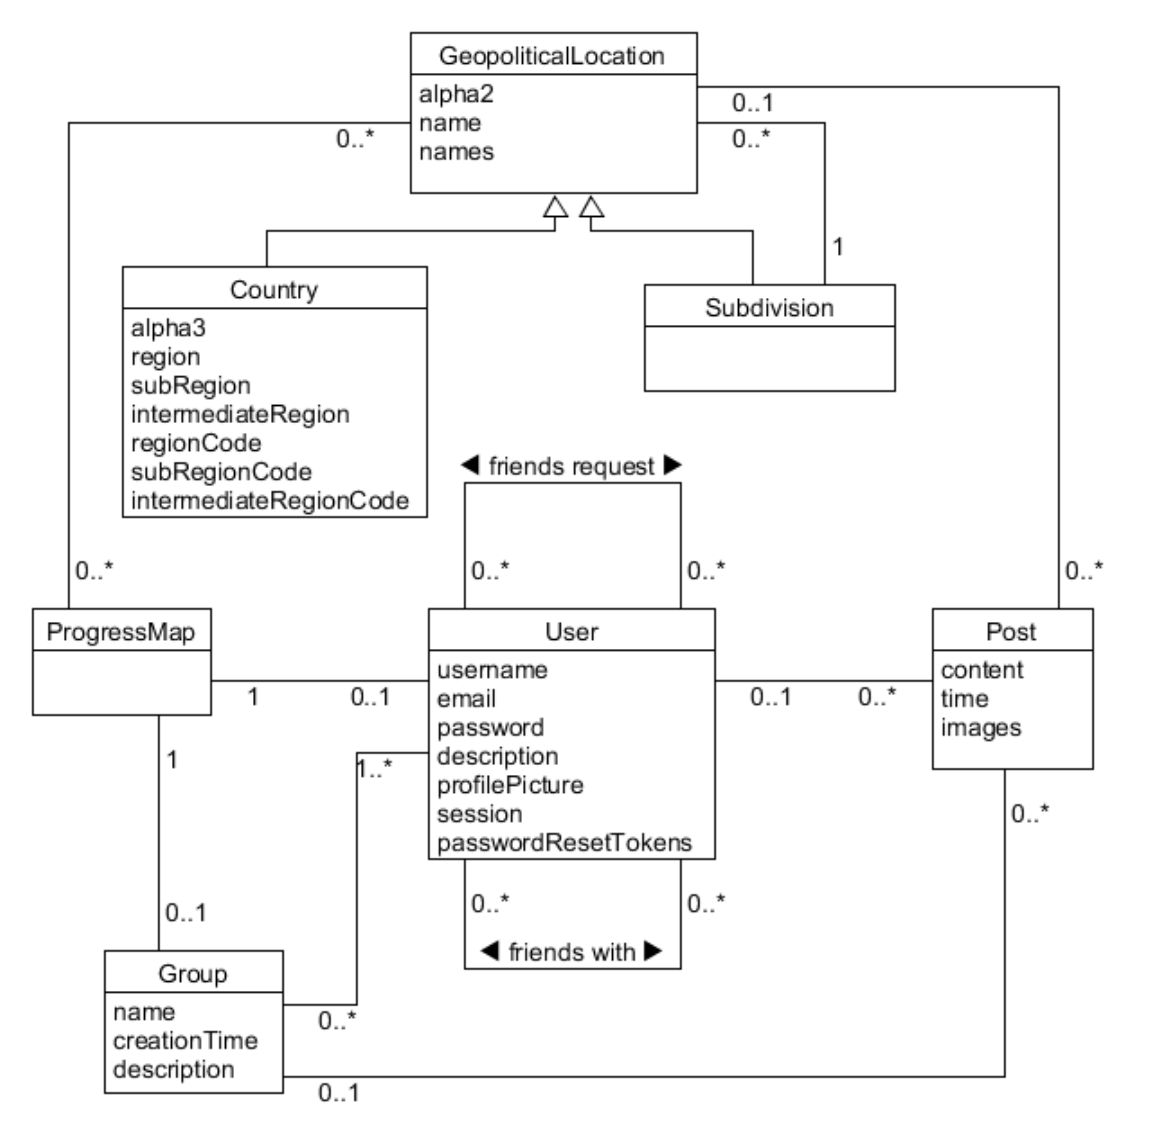
\includegraphics[width=\linewidth]{figures/Domain.png}
    \caption{Domain model}
    \label{fig:Domain}
\end{figure}


 
\begin{figure}
    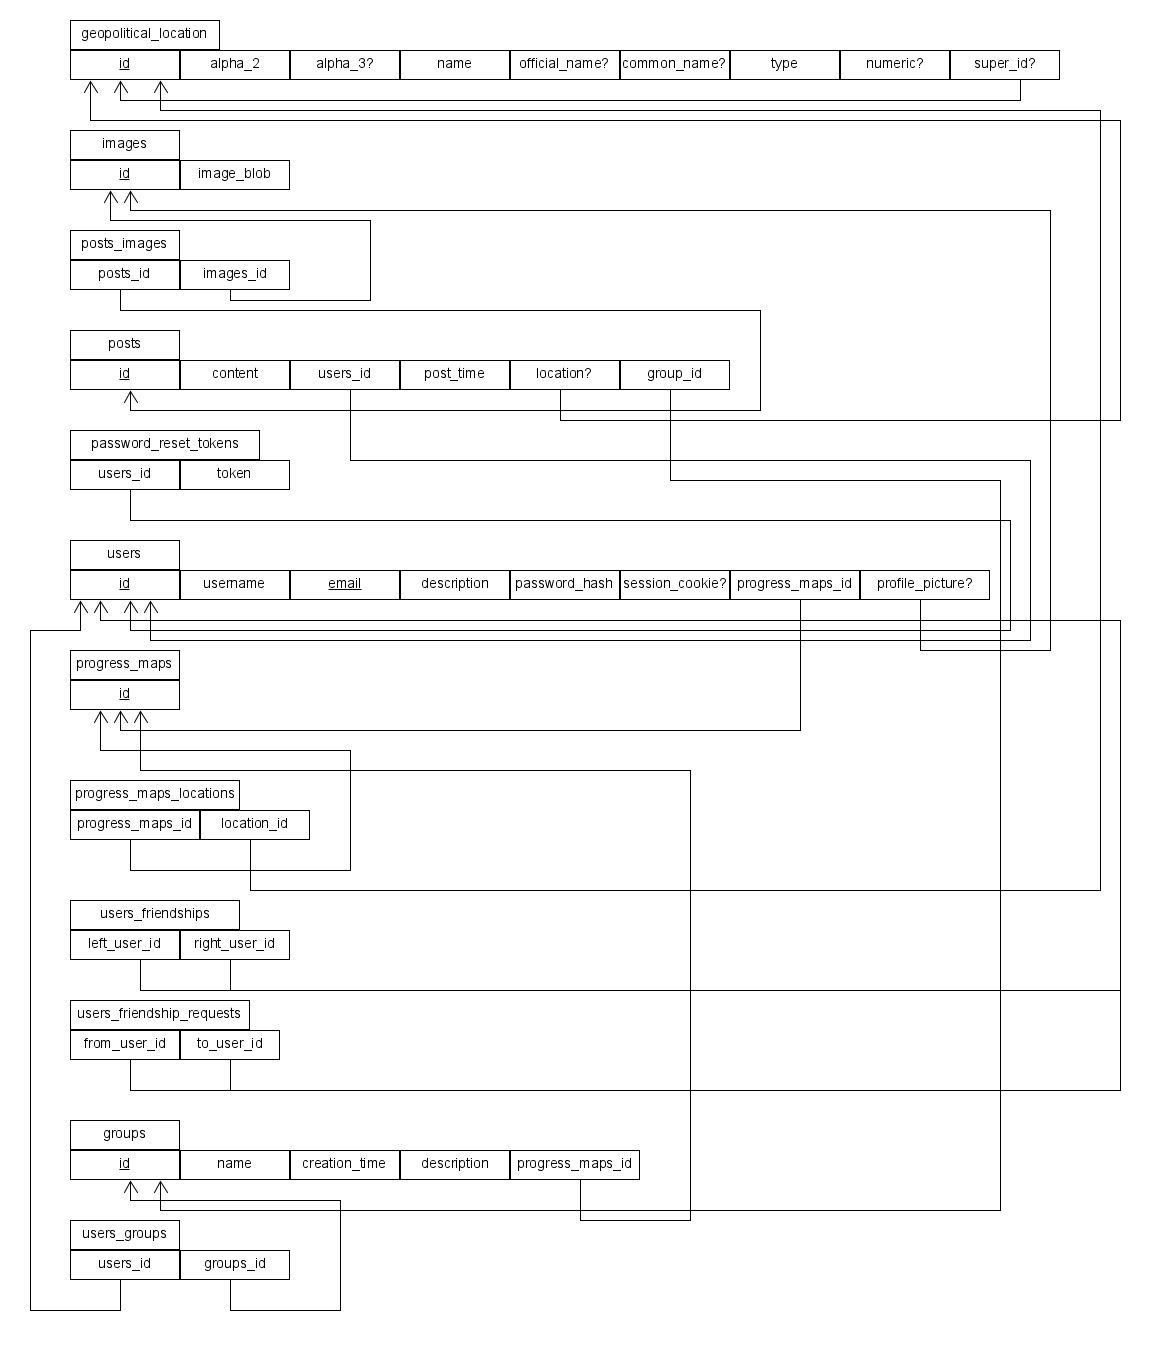
\includegraphics[width=\linewidth]{figures/RelationelmModel.png}
    \caption{Relationel Model}
    \label{fif:Rela}
\end{figure}



\begin{figure}
    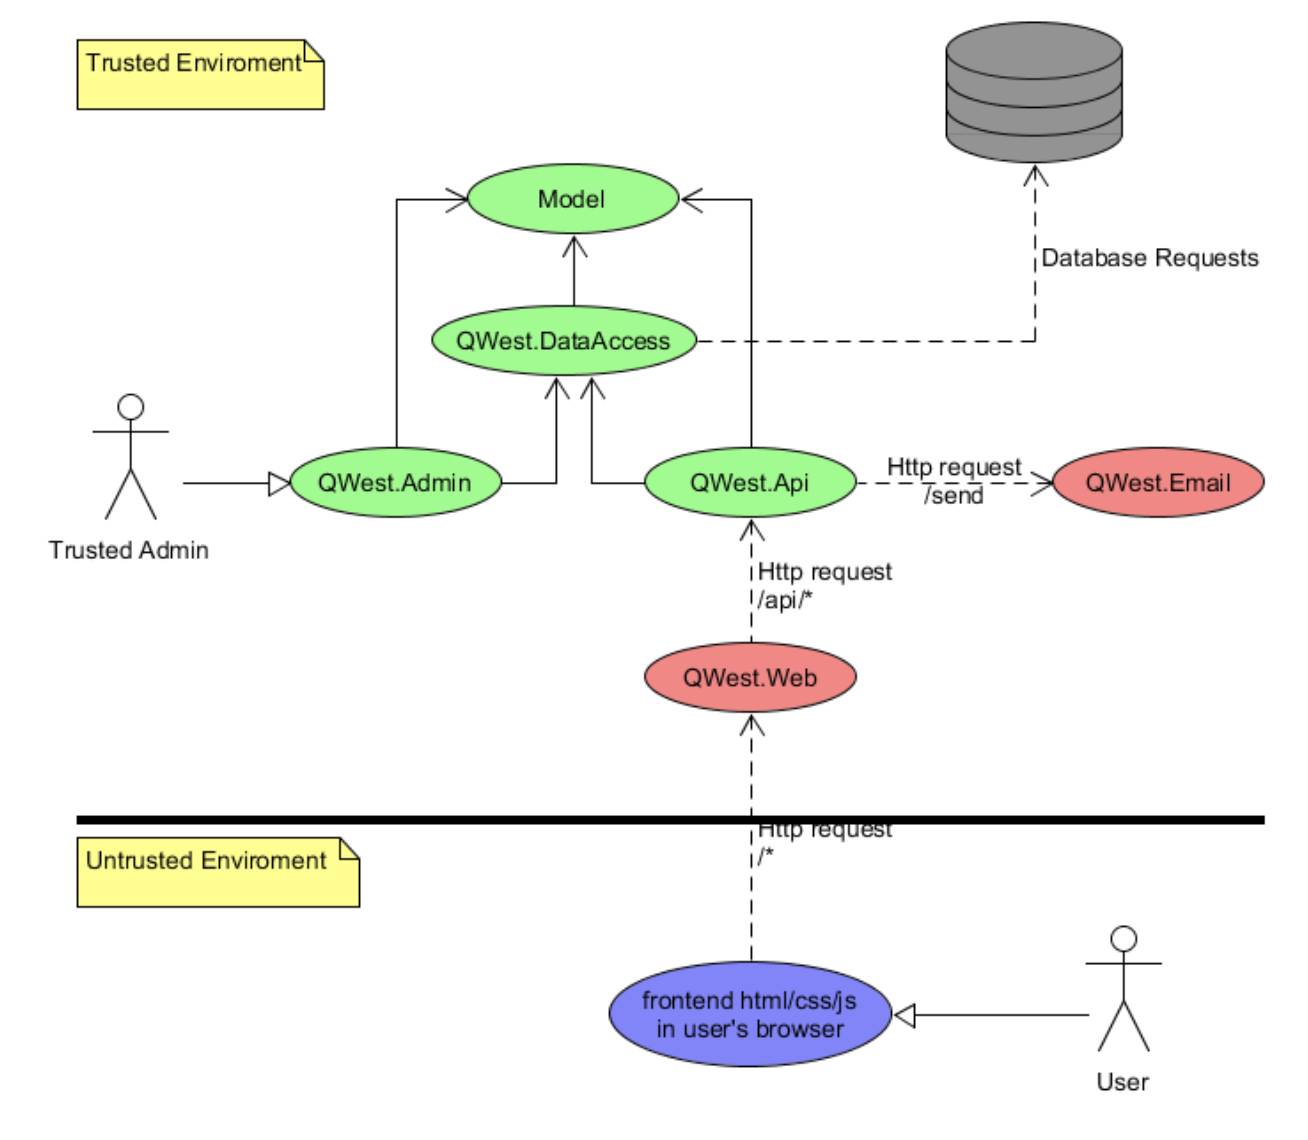
\includegraphics[width=\linewidth]{figures/Systemarkitektur.png}
    \caption{Systema Arkitektur}
    \label{fig:Arki}
\end{figure}


Eftersom system arkitekturen er desigent, kan teamet fokuserer på at udvikle softwaren med respekt til designet. For at skabe den bedst mulige kvaliet af software, har teamet fokuseret på at kvalitetssikre procressen. I næste afsnist vil vi se på hvordan FURPS+ og bestemte XP praktikker er benyttet til at kvalitetssikre produktet. 